Although loading and cooling \ce{Be+} ions is fairly straight forward, it is not as clear as how to load \ce{C+} ions into the trap with \ce{Be+} reliably. Early attempts involved using the home-made electron gun to dissociate \ce{CO} gas introduced via leak valve, where all possible ionized products of \ce{CO} were detected (\ce{C+}, \ce{O+}, and \ce{CO+}). Even when loading into an empty trap, it was not possible to reliably isolate the \ce{C+} via A-ramping of the trap RF voltage. Prolonged use of the electron gun directly towards the ion trap also caused charging that would slowly dissipate and change the trap parameters. On top of these complications, it would not have worked in conjunction with ablation loading \ce{Be+}, as these cannot occur simultaneously.

Instead of using two different methods to load the different ion species, ablating samples of both species simultaneously was found to be the best method. A sample of \ce{Be} metal was placed on top of a piece of graphite on the target holder so that both samples were in view of the ablation laser. The set up shown in figure \ref{fig: dual ablation} allowed us to separate the Minilite ablation laser into two beam with independent alignment and focal planes. The polarization of the laser light is rotated with a half-waveplate, which then enters a polarizing beam splitter (PBS), allowing for tuning of power into either path. The vertically polarized reflected light is reflected off a second PBS and is steered up to the objective lens and then focused into the chamber. The horizontally polarized light transmitted through the first PBS is aligned through an adjustable telescope system. This light is then realigned with the vertically polarized light on the second PBS, co-propagating into the chamber. This "delay stage" for the horizontal light allows for independent focusing and alignment onto a target.

Blocking one beam allowed for adjustments for the ablation of each species independently. When loading \ce{C+}, we found a strong dependence of the trapped species and the fluence. Lower fluence created not only \ce{C+}, but clusters of, \ce{C2+}, and \ce{C3+} as well. Tight focusing of the beam improves the efficiency of creating only \ce{C+}, but some \ce{Cn+} is still usually produced. By changing the trap's $a$ parameter (A-ramp) via changing the $V_{DC}$ (\ref{eq: a param}), we can change the stability diagram for the trap, causing higher $m/z$ ions to become more unstable. The higher mass \ce{Cn+} ions are preferentially kicked out of the trap, while the lighter \ce{Be+} and \ce{C+} are less affected, allowing us to load clean samples of the desired species.

\begin{figure}[H]
	\centering
	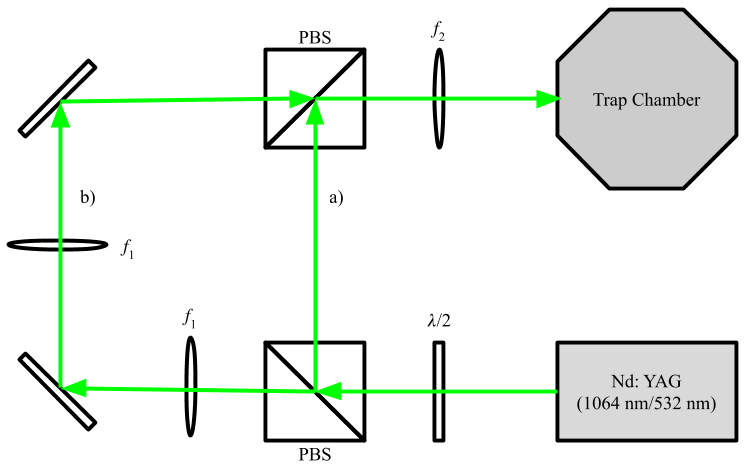
\includegraphics[width=\textwidth]{images/ablation_optics_diagram.png}
	\caption{Diagram of the single laser, dual ablation set up. The 1064 nm/532 nm YAG pulse is split into two paths via polarizing beam splitter (PBS), and recombined such that they proceed through the same focusing element into the chamber to hit two different targets. Path a) is used for the ablation of graphite to produce \ce{C+}, while path b) is independently focused and positioned to ablate beryllium metal to produce \ce{Be+}. The ratio of power in each path is adjusted via the half waveplate directly in front of the laser.}
	\label{fig: dual ablation}
\end{figure}

\begin{figure}[H]
	\centering
	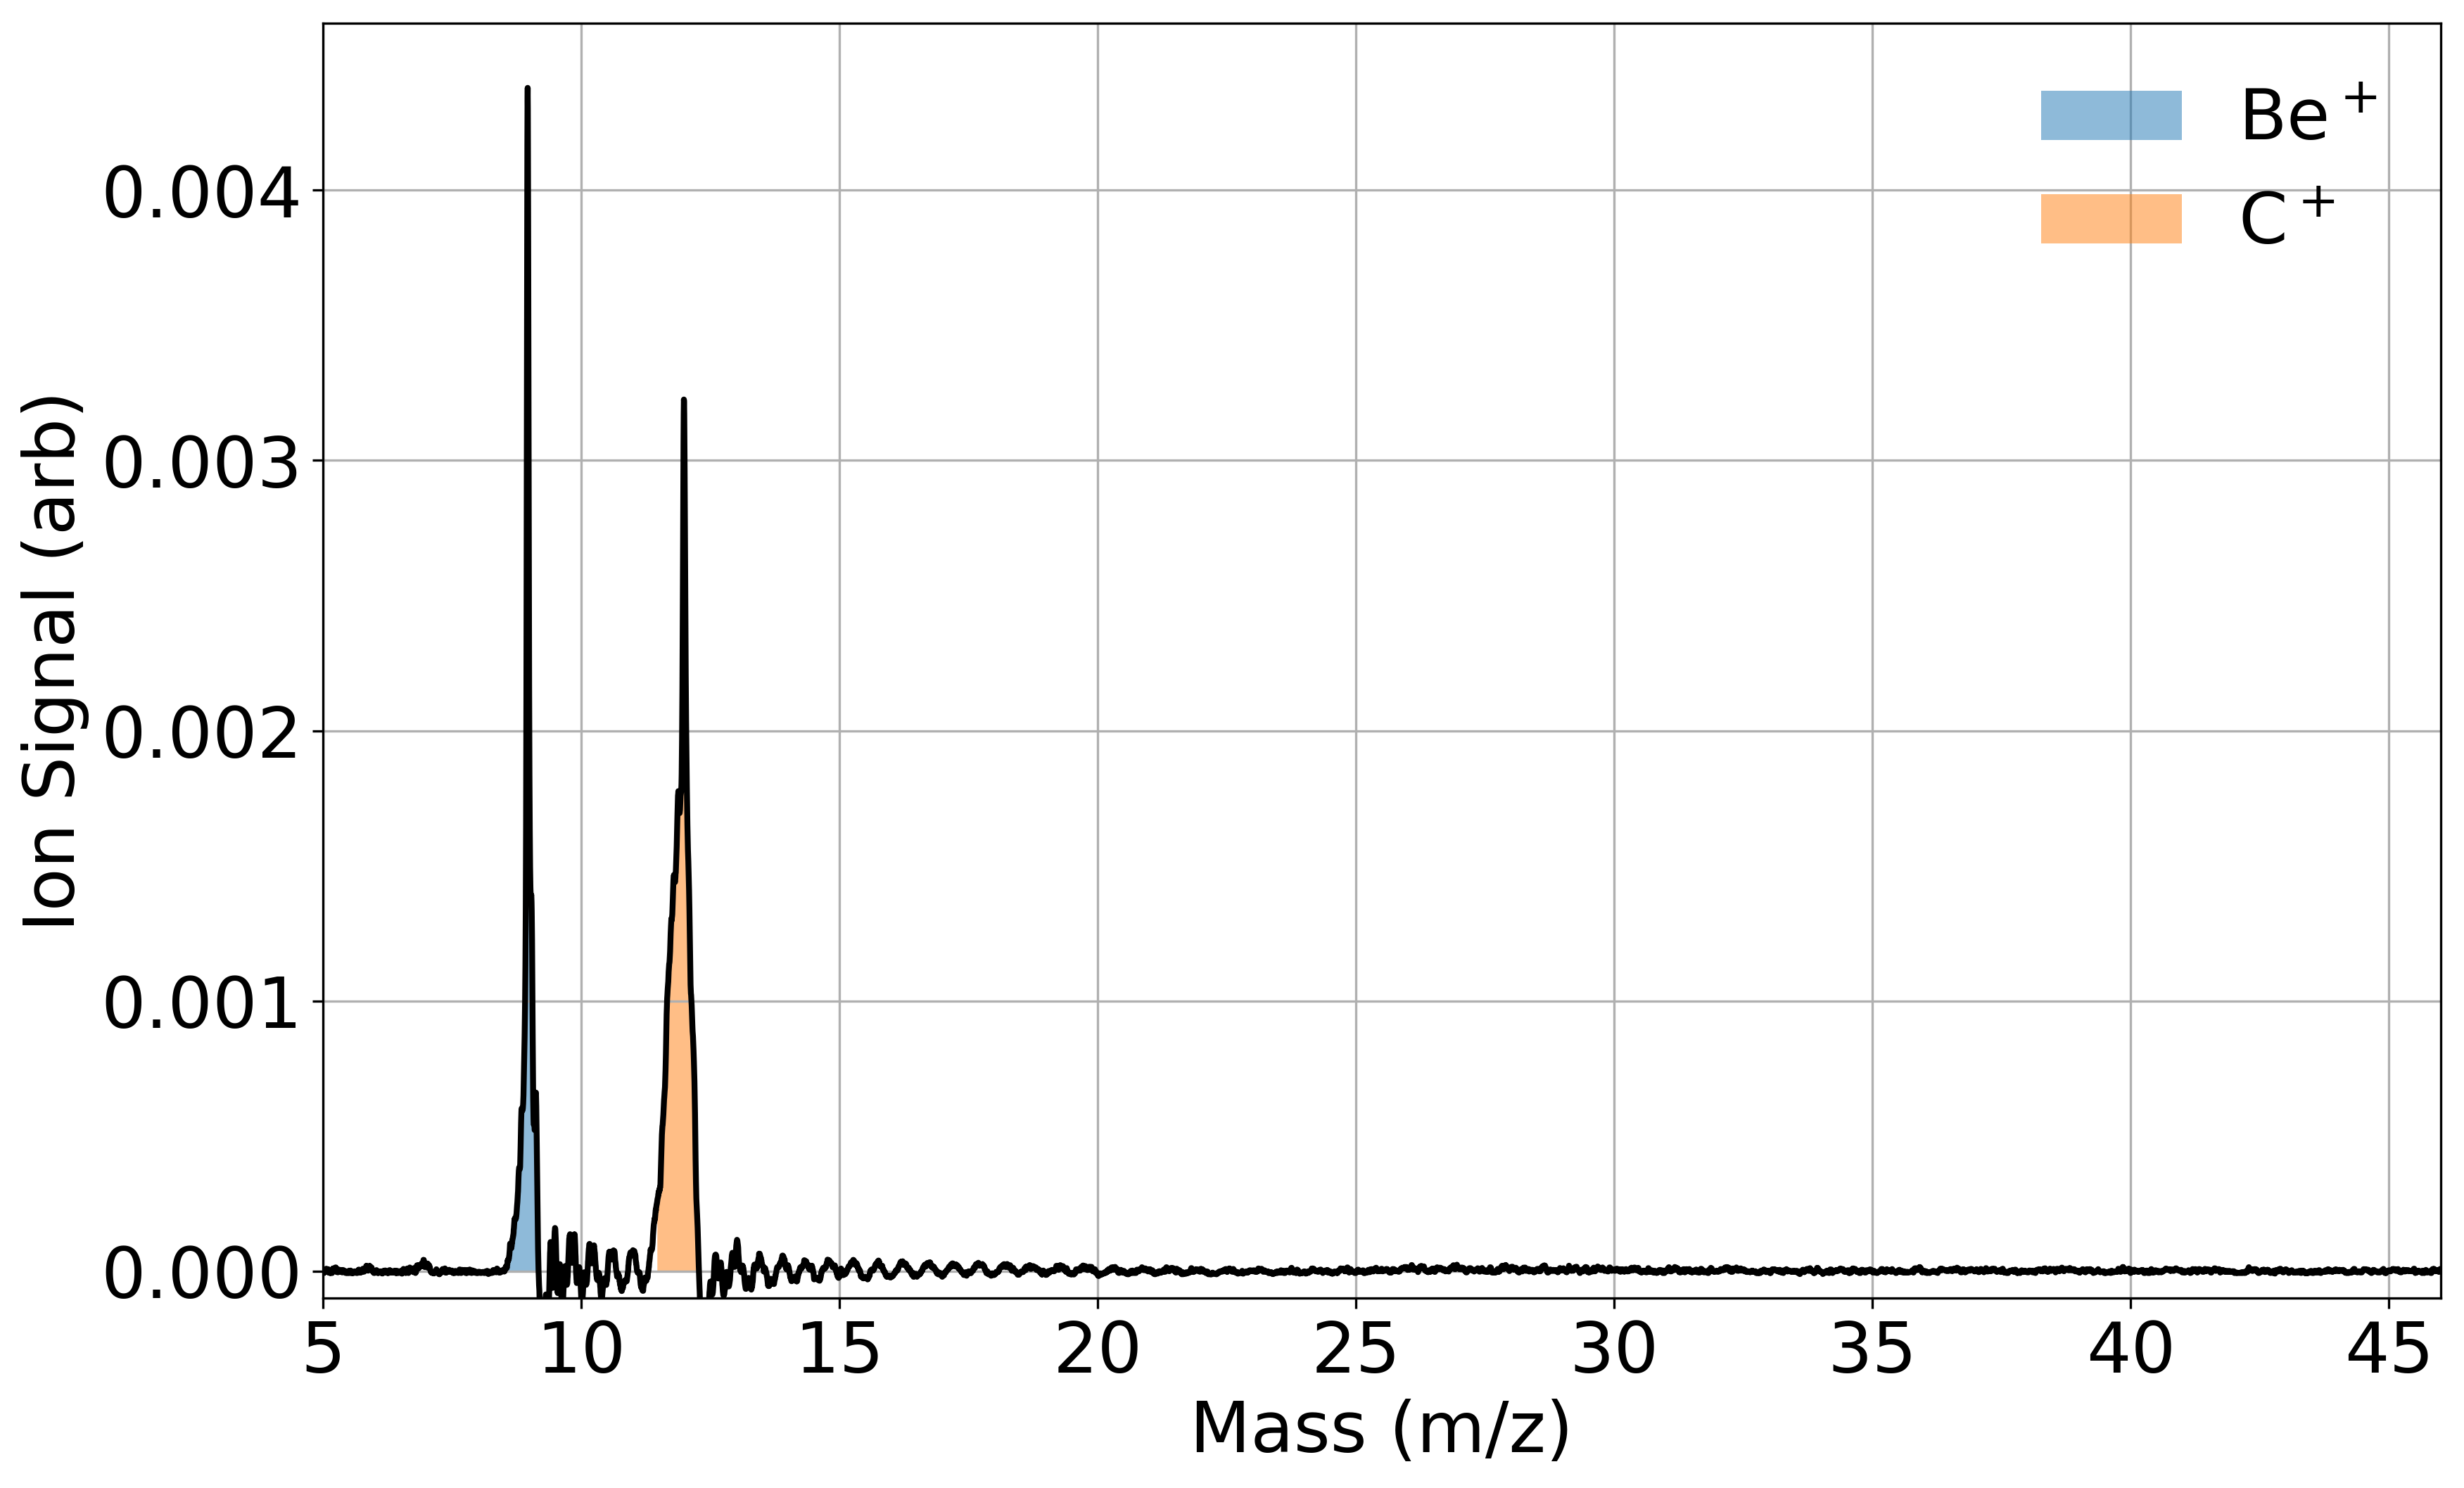
\includegraphics[width=0.8\textwidth]{images/Be_C_TOF.png}
	\caption{TOF trace of simultaneous \ce{Be+} and \ce{C+} ablation loading averaged over 10 shots. A soft A-ramp is applied after loading, ejecting any unintentionally loaded \ce{Cn+} clusters. The \ce{C+} peak is narrowed from sympathetic cooling with the laser cooled \ce{Be+} ions.}
	\label{fig: Be C TOF}
\end{figure}

An important consideration is that that the amount of ions loaded from shot-to-shot is not identical; the amounts may be similar, but can drift over time, especially for the \ce{C+} peak, as the ablation of graphite is less reliable as beryllium metal. As we run experiments, which can take upwards of 200 shots to complete, we cannot make assumptions on the total number or ratio of loaded ions. With \ce{Be+}, we may use the camera in conjunction with the TOF and normalize the total \ce{Be+} reaction network with the fluorescence. Because the \ce{Be+} fluorescence has no indication on the amount of \ce{C+} loaded into the trap, the \ce{C+} reaction network must then be normalized separately for total ion count in each division.